
\section{The Large Hadron Collider}
\label{sec:cmsExperiment:lhc}

% overview
The Large Hadron Collider (LHC) \cite{exhep:lhc:Evans:2008zzb} is a 27km circular particle collider located at the European Organization for Nuclear Research (CERN) across the border between France and Switzerland. The LHC was constructed during 1998-2008 in a 100-meter-deep underground tunnel previously occuplied by the Large Electron–Positron Collider (LEP) \cite{exhep:lep:Myers:1991ym}. Inside the LHC, two proton beams collide at a maximum center-of-mass energy of $\sqrt{s}=14$\TeV with a designed instant luminosity of $10^{34}$\percms. Around the ring path of the LHC, four collision positions are designed for the four LHC experiments: CMS \cite{exhep:cms:Chatrchyan:2008aa} at point-5, ATLAS \cite{exhep:atlas:Aad:2008zzm} at point-1, LHCb \cite{exhep:lhcb:Alves:2008zz} at point-8 and Alice \cite{exhep:alice:Aamodt:2008zz} at point-2.


% constituents
The main components of the LHC include two tubes with ultrahigh vacuum and about ten thousand superconducting magnets with various sizes installed alone the ring. The magnets include 1232 dipole magnets with a length of 15m to bend the beams and 392 quadrupole magnets with a length of 5m-7m to focus the beams \cite{exhep:lhcFactsFigures}. Magnets of higher multipole orders are also used for corrections of the magnetic field. A liquid helium cooling system is used to cool the superconducting electromagnets at a cryogenic temperature of -271.3\si{\degreeCelsius}. 


\begin{figure}[ht]
    \centering
    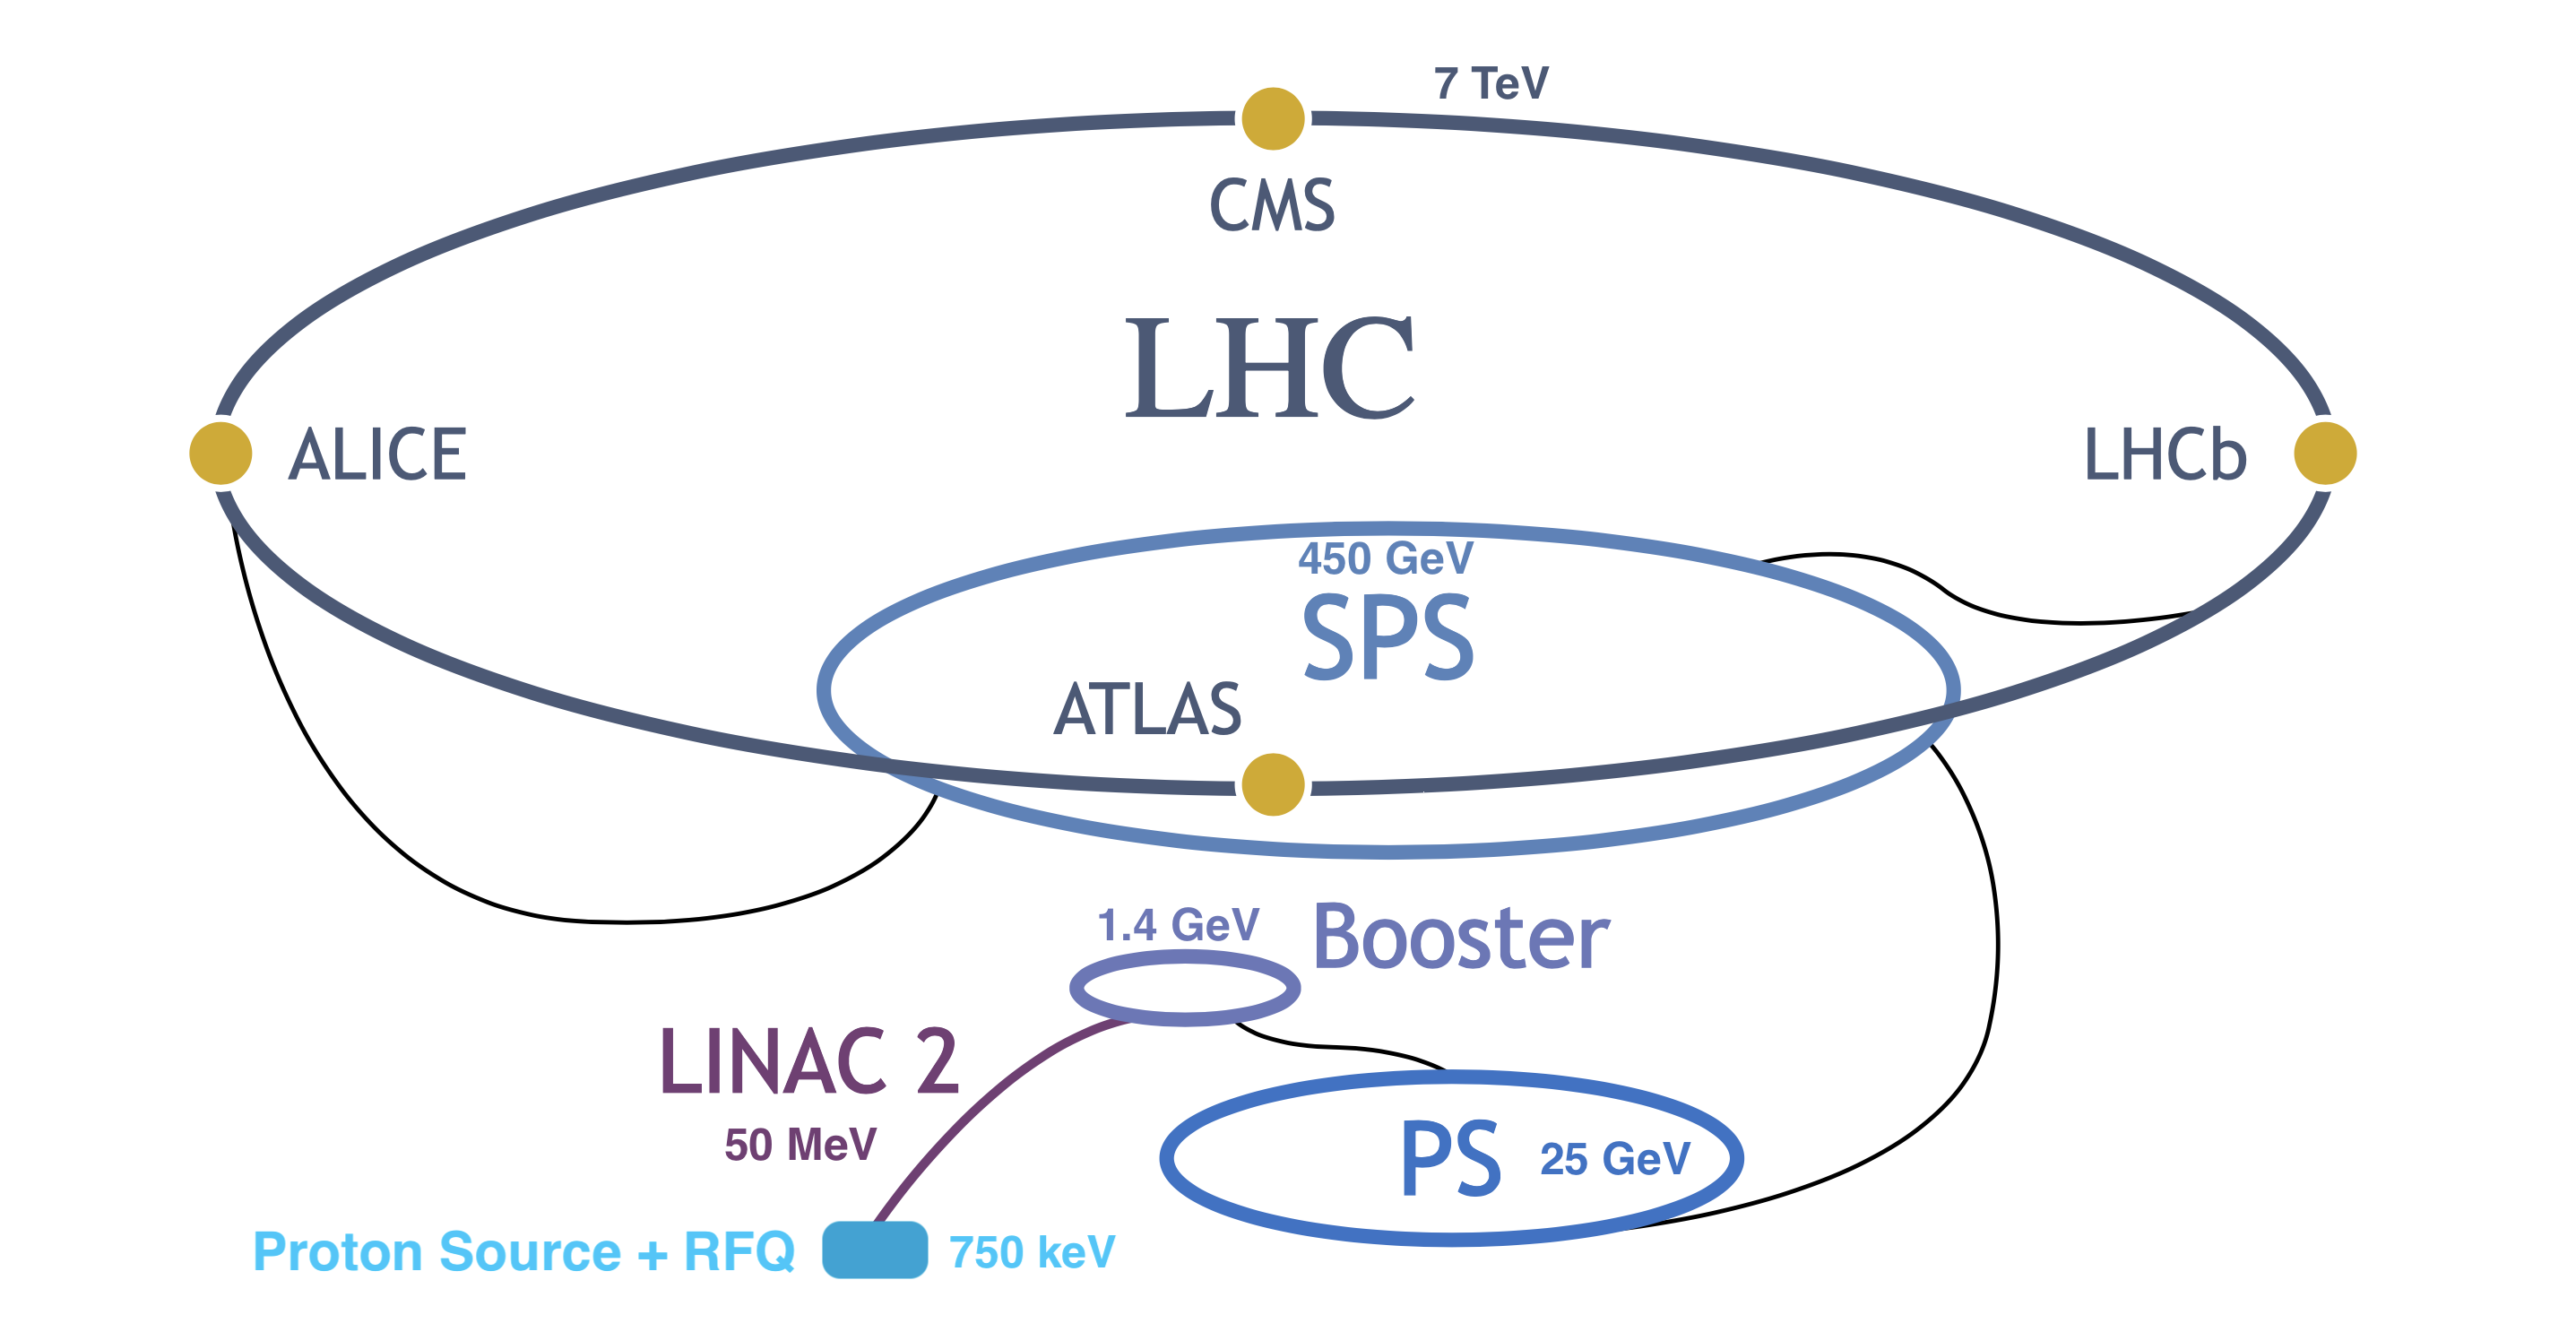
\includegraphics[width=0.8\textwidth]{chapters/CMSExperiment/sectionLHC/figures/lhc.png}
    \caption{Schematic overview of the LHC and the related accelerator complex. The accelerator chain, from the beginning to the end, includes the proton source, radio frequency quadrupole (RFQ), LINAC, proton synchrotron booster (PSB), proton synchrotron (PS), super proton synchrotron (SPS), and finally the LHC \cite{exhep:lhcInject:Benedikt:2004wm}. Around the ring path of the LHC locate four LHC experiments: CMS \cite{exhep:cms:Chatrchyan:2008aa} at point-5, ATLAS \cite{exhep:atlas:Aad:2008zzm} at point-1, LHCb \cite{exhep:lhcb:Alves:2008zz} at point-8 and Alice \cite{exhep:alice:Aamodt:2008zz} at point-2.}
    \label{fig:cmsExperiment:lhc:map}
\end{figure}

% beam pipe
Before injected into the LHC, protons are accelerated to 450\GeV by a few existing accelerator facilities at CERN. Figure~\ref{fig:cmsExperiment:lhc:map} shows a schematic overview of the LHC with its related accelerator complex  \cite{exhep:lhcInject:Benedikt:2004wm}. First, protons are produced by the ionization of the hydrogen gas and extracted by a 90\keV voltage to inject into the radio frequency quadrupole (RFQ), which divides protons into bunch crossings and accelerates them to 750\keV. A linear accelerator (Linac) then energizes them to 50\MeV. The proton synchrotron booster (PSB), which has four superimposed synchrotron rings, brings the proton energy further to 1.4\GeV for the injection to the proton synchrotron (PS), a 628m synchrotron outputting beams with an energy of 25\GeV. The super proton synchrotron (SPS) further boosts the protons to 450\GeV in its 7-km-long ring and delivers the beam to LHC. When the LHC accelerates the protons from 450\GeV at their injection to 6.5\TeV for the physics collision in the run-2, the dipole magnetic field is increased from 0.54T to 7.7T to enhance the banding power to circulating energized beams. During a physics run, luminosity of LHC decays with a lifetime of about 14.9h \cite{exhep:lhc:Evans:2008zzb} due to losses from physics collisions, photon emittances alone the circular path, and the scattering at the air remains. Therefore, new bunches of protons are injected into the LHC every one or two days.



% operation schedule
The operation of the LHC from 2010 to 2035 consists of 6 runs with shutdown periods during the run intervals for upgrade and maintenance . In the run-1 from 2010 to 2013, LHC delivered about 6\fbinv proton-proton collision at $\sqrt{s}=7$\TeV in 2010-2011 and 23.3\fbinv proton-proton collision at $\sqrt{s}=8$\TeV in 2012 \cite{cms:publicLumiInfo}. The discovery of the Higgs boson was made by the ATLAS \cite{exhep:atlasHiggsDisc:Aad:2012tfa} and the CMS \cite{exhep:cmsHiggsDisc:Chatrchyan:2012ufa} during the run-1. In the run-2 from 2016 to 2018, LHC produced 144\fbinv proton-proton collisions at $\sqrt{s}=13$\TeV \cite{cms:publicLumiInfo}. Currently in 2020, the LHC is in its second long shutdown period, expecting Run-3 to start in 2021, operating at the maximum collision energy of $\sqrt{s}=14$\TeV. After run-3, LHC will be upgraded to a higher luminosity or the High-Luminosity LHC (HL-LHC), reaching an instant luminosity of $5 \times 10^{34}$\percms, five times as much as the current value. In the era of HL-LHC, three extra runs are scheduled during 2026-2035. In the long term future beyond the HL-LHC era, the Future Circular Collider (FCC) \cite{exhep:fcc:Benedikt:2715354} plan is proposed to build a 100km hadron collider next to the LHC, further increasing the collision energy to a level of 100\TeV.